\section{Sistema de telemetría}
\label{sec:telemetria}

El sistema de telemetría registra en tiempo real todo lo que ocurre durante una sesión
de producción: cambios de fuente activa, transiciones de composite, activaciones del
stream blanker, estado de overlays y niveles de audio. Esta información permite tanto
monitorizar la sesión mientras está en curso como auditarla en detalle una vez terminada
la emisión.

\subsection{Cómo funciona}

El servicio (\texttt{telemetry\_service.py}) es un proceso independiente que no forma
parte del núcleo de procesamiento. Se conecta a voctocore en el puerto~9999 como un
cliente TCP ordinario y consulta su estado cada segundo. Sin embargo, voctocore solo
conoce lo que ocurre en el mezclador: qué fuente está en programa, qué composite está
activo o cuál es el estado del stream blanker. Todo lo que gestiona la interfaz gráfica,
como las fuentes seleccionadas en preview, los niveles de audio o los overlays activos,
queda fuera de su alcance.

Para capturar también este segundo bloque de información, el módulo
\texttt{gui\_state\_exporter.py} de voctogui exporta el estado completo de la interfaz
gráfica cada segundo. En el escenario de un PC lo escribe en un fichero local
(\texttt{sessions/gui\_state.json}); en escenarios con red (Docker o dos PCs) lo envía
directamente al servicio mediante una petición HTTP POST al puerto~8080. Esta última
opción, basada en HTTP, sustituyó a una implementación inicial con UDP que presentaba
problemas de pérdida de paquetes y bloqueos de puerto al reiniciar los scripts durante
el desarrollo.

El servicio fusiona las dos fuentes de información y construye una vista unificada de la
sesión, que guarda en formato \textit{JSON Lines}
(\texttt{sessions/session\_N.jsonl}): un objeto JSON completo por línea, con numeración
automática por sesión. Este formato permite analizar el log de forma incremental con
herramientas estándar como \texttt{jq} o Python, sin necesidad de cargar el fichero
completo en memoria.

\begin{figure}[H]
  \centering
  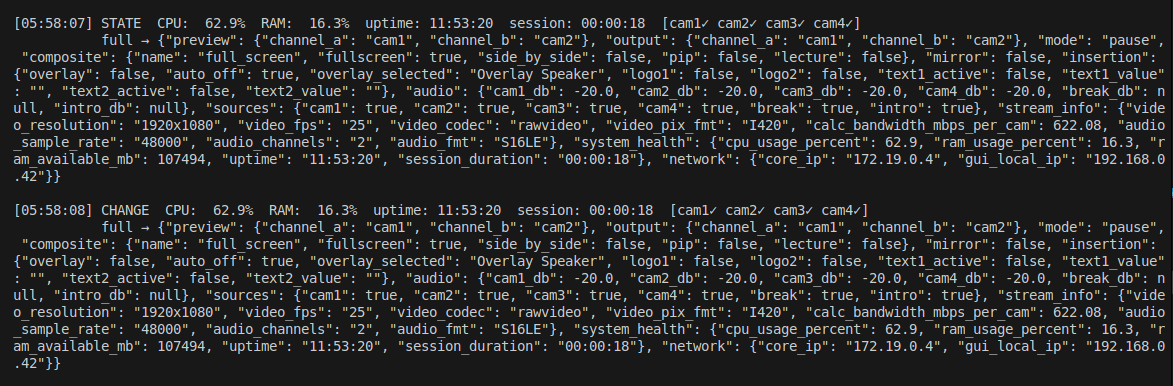
\includegraphics[width=\textwidth]{figuras/telemetria_state_change.png}
  \caption{Salida del servicio de telemetría mostrando un evento STATE y un evento
           CHANGE consecutivos durante una sesión real.}
  \label{fig:telemetria_state_change}
\end{figure}

\subsection{Tipos de entrada: Change y State}

El registro combina dos tipos de entrada:

\begin{itemize}
  \item \textbf{Evento Change (\texttt{CHANGE}):} se escribe inmediatamente cuando se
        detecta cualquier variación de estado, como un corte de cámara o un cambio de
        composite. Captura el instante exacto en que ocurre el cambio.
  \item \textbf{Evento State (\texttt{STATE}):} un hilo independiente escribe el estado
        completo del sistema cada 5~segundos, con independencia de que haya habido
        cambios. Sirve como mecanismo de redundancia para poder reconstruir la sesión
        aunque se pierda algún evento.
\end{itemize}

Cada entrada incluye la marca de tiempo, el estado de todas las fuentes, el composite
activo, el modo de stream (LIVE, PAUSE o NOSTREAM), los overlays y los niveles de audio
en decibelios. Se añade además un bloque \texttt{system\_health} con el uso de CPU y RAM
del servidor, lo que permite relacionar eventuales degradaciones de la señal con picos
de carga del sistema. El campo \texttt{stream\_info} almacena los parámetros técnicos
del pipeline: resolución, framerate, formato de píxel y el ancho de banda calculado por
fuente (622~Mbps para 1080p25 en I420).

Un ejemplo de entrada de tipo CHANGE tras un corte de cámara:

\begin{verbatim}
{"timestamp": "2025-03-28 20:14:32",
 "type": "change",
 "output":  {"channel_a": "cam2", "channel_b": "cam1"},
 "preview": {"channel_a": "cam1", "channel_b": "cam2"},
 "mode": "live",
 "composite": {"name": "full_screen", "fullscreen": true},
 "audio": {"cam1_db": -12.0, "cam2_db": 0.0},
 "system_health": {"cpu_usage_percent": 34.2, "ram_usage_percent": 8.7,
                   "calc_bandwidth_mbps_per_cam": 622.08},
 "stream_info": {"video_resolution": "1920x1080", "video_fps": "25",
                 "video_pix_fmt": "I420"}}
\end{verbatim}

\subsection{API HTTP y publicación en RabbitMQ}
\label{sec:rabbitmq}

Además del fichero de log local, el servicio expone una API HTTP en el puerto~8080 que
devuelve el estado actual completo en formato JSON. Esto permite que otros procesos del
sistema consulten el estado de la sesión en cualquier momento sin acceder directamente
al log.

Opcionalmente, el servicio puede publicar cada evento en un broker
RabbitMQ~\cite{rabbitmq_docs} mediante el protocolo AMQP~\cite{oasis_amqp10}. Cada
cambio de estado se publica en el exchange \texttt{voctomix\_events} (tipo fanout), de
forma que cualquier consumidor externo puede suscribirse a los eventos sin acoplarse
directamente al servicio de telemetría ni a voctocore. Si RabbitMQ no está disponible,
el servicio continúa funcionando con el log local y la API HTTP sin interrupción alguna.

En el marco del proyecto europeo CyberNEMO (UPM), el broker RabbitMQ de Voctomix~2.0
fue integrado en el clúster Kubernetes del proyecto, donde las colas
\texttt{vproduction-uc-media} y \texttt{vqprobe-uc-media} recibieron los eventos del
mezclador en tiempo real durante las pruebas de producción audiovisual. Este despliegue
constituyó la primera validación del sistema de telemetría en un entorno real.

\begin{figure}[h]
  \centering
  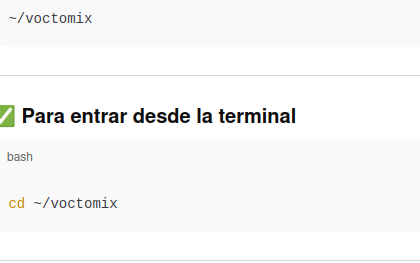
\includegraphics[width=\textwidth]{figuras/rabbitmq_cybernemo_queues.png}
  \caption{Colas RabbitMQ activas durante la integración con CyberNEMO.}
  \label{fig:rabbitmq_cybernemo}
\end{figure}

La arquitectura desacoplada del servicio, conectado al núcleo como un cliente TCP
ordinario sin privilegios especiales, garantiza que un eventual fallo del servicio de
telemetría no afecte al procesamiento multimedia principal.
